%------------------------------------------------------------------------%
% Thesis template for the College of Arts & Sciences at Dartmouth        % 
% College. Properties of the final document conform to the 2013 edition  %
% of the thesis guidelines document.                                     %
%                                                                        %
%      Author: Gregory Alexander Feiden                                  %
%   Institute: Dartmouth College                                         %
%        Date: 2014 May 17                                               %
%                                                                        %
%     License: Beerware (revision 42)                                    %
%              ----------------------                                    %
%              Gregory Feiden wrote this file. As long as you retain     %
%              this notice you can do whatever you want with this code.  %
%              If we meet some day and you think this code is worth it,  %
%              you can buy me a beer in return.                          %
%                                                                        %
%------------------------------------------------------------------------%

\documentclass[12pt]{report}

%--- BEGIN HEADER
\usepackage{natbib}
\usepackage[left=1.5in, right=1in, top=1in, bottom=1in]{geometry}
\usepackage{amsmath}
\usepackage{amssymb}
\usepackage{amsfonts}
\usepackage[dvips]{graphicx}
\usepackage{pslatex}
\usepackage{epsfig}
\usepackage{longtable}
\usepackage{lscape}
\usepackage{setspace}
\usepackage{parskip}
\usepackage{listings}
\usepackage[usenames,dvipsnames]{xcolor}
\usepackage[labelfont=bf]{caption}

% use Linux Libertine font package
\usepackage{inconsolata}
\usepackage{fourier}
\usepackage{libertine}
\renewcommand*\oldstylenums[1]{{\fontfamily{fxlj}\selectfont #1}}
\usepackage[T1]{fontenc}

% define how code will appear using listings
\lstset{frame=tb,
  aboveskip=3mm,
  belowskip=3mm,
  showstringspaces=false,
  columns=flexible,
  basicstyle={\small\ttfamily},
  numbers=none,
  numberstyle=\tiny\color{Gray},
  keywordstyle=\color{Maroon},
  commentstyle=\color{MidnightBlue},
  stringstyle=\color{Magenta},
  breaklines=true,
  breakatwhitespace=true
  tabsize=4
}

% Use hyperref to allow for interal and external hyperlinking
\usepackage[pdftex]{hyperref}
\hypersetup {
    bookmarks=true,                    % show bookmarks bar in pdf reader
    pdftitle={},                       % set pdf title
    pdfauthor={},                      % set pdf author
    pdfsubject={},                     % pdf subject
    colorlinks=true,                   % false = box link, true = colored links
    linkcolor=blue,                    % color of internal links
    citecolor=blue,                    % color of citations
    urlcolor=blue                      % external url color
}
\urlstyle{same}

\pagestyle{plain}                  % page number at bottom-center of page
\citestyle{aa}                     % A&A citation style (removes comma)
\doublespacing                    % Thesis must be doubled spaced

% Configure how figure + table captions will appear
\captionsetup[table]{textfont=sc, labelsep=newline, labelformat=simple,
                       justification=centering}
\captionsetup[figure]{textfont=normalfont, labelsep=colon, labelformat=simple}

% Make figures and tables labeled by chapter.number
\renewcommand{\thefigure}{\thechapter.\arabic{figure}}
\renewcommand{\thetable}{\thechapter.\arabic{table}}

%--- END HEADER

%--- NEW COMMANDS SECTION
% thermodynamic derivatives (partial and total)
\newcommand{\thermt}[4] {\left(\frac{d #1}{d #2}\right)_{#3,#4}}
\newcommand{\thermd}[4] {\left(\frac{\partial #1}{\partial #2}\right)_{#3,#4}}
\newcommand{\el}[2]{$^{#1}$#2}                 % Isotope formatting
\newcommand{\msun}{M_{\odot}}                 % Solar mass
\newcommand{\rsun}{R_{\odot}}                 % Solar radius
\newcommand{\lsun}{L_{\odot}}                 % Solar luminosity
\newcommand{\teff}{T_{\rm eff}}               % Effective temperature
\newcommand{\porb}{P_{\rm orb}}               % Orbital period
\newcommand{\amlt}{\alpha_{\rm MLT}}         % Mixing length parameter 
\newcommand{\grad}{{\bf \nabla}}             % Gradient vector
\newcommand{\dela}{\nabla_{\rm ad}}          % Adiabatic gradient
\newcommand{\delr}{\nabla_{\rm rad}}         % Radiative gradient inhibition
%For astronomers, you might find that some of the familiar symbols from aastex is not availabe
%In these situations, download aastex.cls from https://aas.org/aastex/aastex-downloads
%and locate your favorite commands in it
%Here's a few example
\newcommand\micron{\mbox{$\mu$m}}             %micron symbol
\newcommand{\arcdeg}{\ensuremath{^{\circ}}}   % degree symbol:  °
\newcommand\arcsec{\mbox{$^{\prime\prime}$}}  % arcsecond symbol
% Journal abbreviations might also come in handy
\newcommand{\apj}{ApJ}
\newcommand{\apjs}{ApJS}
\newcommand{\apjl}{ApJL}
\newcommand{\aap}{A{\&}A}
\newcommand{\aaps}{A{\&}AS}
\newcommand{\mnras}{MNRAS}
\newcommand{\aj}{AJ}
\newcommand{\araa}{ARAA}
\newcommand{\pasp}{PASP}
%--- END NEW COMMANDS SECTION


%--- CITATION ALIASES
% define all citation alias (shorthand versions for in-text citations)
%   ex: \defcitealias{CITEKEY}{Paper I} 

%--- END CITATION ALIASES


%--- BEGIN THESIS DOCUMENT
\begin{document}

% Note: chapters are all contained in separate files in subdirectories. 
%       They are called using '\include' instead of '\input' so that 
%       they will begin on a new page.

%------------------------------------------------------------------------%
% Front matter for Ph.D. thesis, incl., title page, copyright, preface,  %
% table of contents, list of tables, and list of figures.                %
%                                                                        %
%      Author: Gregory Alexander Feiden                                  %
%   Institute: Dartmouth College                                         %
%        Date: 2014 May 17                                               %
%                                                                        %
%     License: Beerware (revision 42)                                    %
%              ----------------------                                    %
%              Gregory Feiden wrote this file. As long as you retain     %
%              this notice you can do whatever you want with this code.  %
%              If we meet some day and you think this code is worth it,  %
%              you can buy me a beer in return.                          %
%                                                                        %
%------------------------------------------------------------------------%

% Create custom title page to conform to 2013 Dartmouth Graduate Office 
% standards.

\begin{titlepage}
 \begin{center}
  \MakeUppercase{\bf title of your thesis} \\ % Note: Call it what you will.
  A Thesis                 \\
  Submitted to the Faculty \\
  in partial fulfillment of the requirements for the \\
  degree of              \\
  Doctor of Philosophy   \\   % Note: Modify to say what degree you're earning.
  in                     \\
  Physics and Astronomy  \\   % Note: And in what field.
  by                     \\
  First Middle Sirname   \\   % Note: You should change this to your name.
  DARTMOUTH COLLEGE      \\
  Hanover, New Hampshire \\
  \today
 \end{center}
 \vspace{\baselineskip}
 
 %\vspace*{0.7in}
 \vspace*{\fill}
 
 \begin{minipage}[b]{\linewidth}
 
    \begin{flushright}
        
        \begin{minipage}[b]{0.45\linewidth}
            \begin{center}
                Examining Committee:
            \end{center}
            \vspace{0.5in}
            \hrule \vspace{0.1in}
            Brian C. Chaboyer (Chair) \\ \vspace{0.3in} % internal #1
            \hrule \vspace{0.1in}
            Robert A. Fesen \\ \vspace{0.3in}           % internal #2
            \hrule \vspace{0.1in}
            John R. Thorstensen \\ \vspace{0.3in}       % internal #3
            \hrule \vspace{0.1in} 
            External E. External                        % external member
        \end{minipage}
    \end{flushright}
 
    \begin{flushleft}
        \vspace*{-0.44in}
        \singlespacing
        \begin{minipage}[b]{0.45\linewidth}
            \hrule \vspace{0.1in}
            F. Jon Kull \\              % check it's the same person
            Dean of Graduate Studies
        \end{minipage}
    \end{flushleft}
    
 \end{minipage}
 
\end{titlepage}

%---BEGIN ROMAN NUMERAL PAGE NUMBERING
\pagenumbering{roman}

% License page. Choose one wisely. If you're unsure, ask a librarian or 
% just use the standard copyright.
\newpage
\thispagestyle{empty}
\begin{center}
    \vspace*{\fill}
    Copyright \copyright\ \the\year\ by Author A. Author \\ 
    This work is licensed under the Creative Commons Attribution 3.0 Unported License. \\
    To view a copy of this license, visit \url{http://creativecommons.org/licenses/by/3.0/}.
    \vspace*{\fill}
\end{center}

% Abstract (on new page)
\newpage
%------------------------------------------------------------------------%
% Abstract formatting for a thesis.                                      %
%                                                                        %
%      Author: Gregory Alexander Feiden                                  %
%   Institute: Dartmouth College                                         %
%        Date: 2014 May 17                                               %
%                                                                        %
%     License: Beerware (revision 42)                                    %
%              ----------------------                                    %
%              Gregory Feiden wrote this file. As long as you retain     %
%              this notice you can do whatever you want with this code.  %
%              If we meet some day and you think this code is worth it,  %
%              you can buy me a beer in return.                          %
%                                                                        %
%------------------------------------------------------------------------%

\vspace*{1in}
{\Huge \bf Abstract} \\

Enter your abstract here.

\addcontentsline{toc}{chapter}{Abstract}

% Preface (including acknowledgements)
\newpage
\addcontentsline{toc}{chapter}{Preface}
%------------------------------------------------------------------------%
% Preface for thesis.                                                    %
%                                                                        %
%      Author: Gregory Alexander Feiden                                  %
%   Institute: Dartmouth College                                         %
%        Date: 2014 May 17                                               %
%                                                                        %
%     License: Beerware (revision 42)                                    %
%              ----------------------                                    %
%              Gregory Feiden wrote this file. As long as you retain     %
%              this notice you can do whatever you want with this code.  %
%              If we meet some day and you think this code is worth it,  %
%              you can buy me a beer in return.                          %
%                                                                        %
%------------------------------------------------------------------------%
%\vspace*{1in}

%---BEGIN INSPIRATION QUOTE 
\begin{flushright}
\begin{minipage}[]{0.55\linewidth}
{\small \emph{Looking back to all that has occurred to me since that eventful
day, I am scarcely able to believe in the reality of my adventures. They 
were truly so wonderful that even now I am bewildered when I think of them.}}
    \begin{flushright}
        {\small \emph{--- Jules Verne} \hspace{0.5in} }
    \end{flushright}
\end{minipage}
\end{flushright}
%\vspace{\baselineskip}
%---END INSPIRATIONAL QUOTE

{\Huge \bf Preface} \\

Gush about everyone, here.




% THERE IS NO NEED TO CHANGE THIS
% Table of contents, list of tables + figures
{
    \newpage
    \hypersetup{linkcolor=black}
    \addcontentsline{toc}{chapter}{Contents}
    \tableofcontents
    
    \newpage
    \addcontentsline{toc}{chapter}{List of Tables}
    \listoftables

    \newpage
    \addcontentsline{toc}{chapter}{List of Figures}
    \listoffigures
}
   % Front Matter: title, preface, abstract, etc.

\pagenumbering{arabic}           % Switch to arabic page numbering for chapters
\doublespacing                   % Document must be double spaced for Dartmouth

%--- ADD CHAPTERS
%------------------------------------------------------------------------%
% Example chapter for the thesis template.                               %
%                                                                        %
%      Author: Gregory Alexander Feiden                                  %
%   Institute: Dartmouth College                                         %
%        Date: 2014 May 17                                               %
%                                                                        %
%     License: Beerware (revision 42)                                    %
%              ----------------------                                    %
%              Gregory Feiden wrote this file. As long as you retain     %
%              this notice you can do whatever you want with this code.  %
%              If we meet some day and you think this code is worth it,  %
%              you can buy me a beer in return.                          %
%                                                                        %
%------------------------------------------------------------------------%

\chapter{Introduction}
\label{chp:intro}

\emph{It was a dark and stormy night, so he decided to be a theorist.}

A nice long introduction with many, many sections and billions of 
citations.
    
    % SECTION: EXAMPLE OF ADDING A SECTION
    %------------------------------------------------------------------------%
% Example section for thesis template.                                   %
%                                                                        %
%      Author: Gregory Alexander Feiden                                  %
%   Institute: Dartmouth College                                         %
%        Date: 2014 May 17                                               %
%                                                                        %
%     License: Beerware (revision 42)                                    %
%              ----------------------                                    %
%              Gregory Feiden wrote this file. As long as you retain     %
%              this notice you can do whatever you want with this code.  %
%              If we meet some day and you think this code is worth it,  %
%              you can buy me a beer in return.                          %
%                                                                        %
%------------------------------------------------------------------------%

\section{Section Title}
\label{sec:section1}
So begins a section. Oh, look, a nice table to go with it.

%------------------------------------------------------------------------%
% Example of a standard table for the thesis template.                   %
%                                                                        %
%      Author: Gregory Alexander Feiden                                  %
%   Institute: Dartmouth College                                         %
%        Date: 2014 May 17                                               %
%                                                                        %
%     License: Beerware (revision 42)                                    %
%              ----------------------                                    %
%              Gregory Feiden wrote this file. As long as you retain     %
%              this notice you can do whatever you want with this code.  %
%              If we meet some day and you think this code is worth it,  %
%              you can buy me a beer in return.                          %
%                                                                        %
%------------------------------------------------------------------------%


\renewcommand{\arraystretch}{1.25}
\begin{table}[t]
    \begin{center}
        \caption[Example of a simple table]
        {An example table formatted to look rather nice, in my opinion.
        Note, use the \newline command to get a second line.}
        \label{tab:ex1}
        \begin{tabular*}{\linewidth}{@{\extracolsep{\fill}} c r c c c c c c c}
        \hline
        \hline\noalign{\smallskip}
        Mass ($\msun$) & [Fe/H] & 0.5 & 1.0 & 2.0 & 3.0 & 4.0 & 5.0 & 10.0 \\
        \noalign{\smallskip}\hline\noalign{\smallskip}
        0.15      & $-0.50$ & 0.1561 & 0.1561 & 0.1561 & 0.1561 & 0.1560 & 0.1560 & 0.1560 \\
        $\vdots$  & $ 0.00$ & 0.1560 & 0.1560 & 0.1560 & 0.1560 & 0.1560 & 0.1560 & 0.1559 \\
        $\vdots$  & $+0.15$ & 0.1557 & 0.1557 & 0.1557 & 0.1557 & 0.1556 & 0.1556 & 0.1556 \\
        0.20      & $-0.50$ & 0.1523 & 0.1523 & 0.1522 & 0.1522 & 0.1522 & 0.1522 & 0.1521 \\
        $\vdots$  & $ 0.00$ & 0.1521 & 0.1521 & 0.1521 & 0.1521 & 0.1521 & 0.1520 & 0.1519 \\
        $\vdots$  & $+0.15$ & 0.1518 & 0.1517 & 0.1517 & 0.1517 & 0.1517 & 0.1517 & 0.1516 \\
        0.25      & $-0.50$ & 0.1499 & 0.1498 & 0.1498 & 0.1498 & 0.1498 & 0.1497 & 0.1496 \\
        $\vdots$  & $ 0.00$ & 0.1496 & 0.1496 & 0.1496 & 0.1496 & 0.1495 & 0.1495 & 0.1494 \\
        $\vdots$  & $+0.15$ & 0.1496 & 0.1496 & 0.1496 & 0.1495 & 0.1495 & 0.1495 & 0.1493 \\
        0.30      & $-0.50$ & 0.1482 & 0.1482 & 0.1481 & 0.1481 & 0.1481 & 0.1480 & 0.1479 \\ 
        $\vdots$  & $ 0.00$ & 0.1480 & 0.1480 & 0.1479 & 0.1479 & 0.1478 & 0.1478 & 0.1477 \\
        $\vdots$  & $+0.15$ & 0.1479 & 0.1479 & 0.1479 & 0.1478 & 0.1478 & 0.1477 & 0.1476 \\
        \noalign{\smallskip}\hline
        \end{tabular*}
    \end{center}
\end{table}


And a nice figure! How lovely.

%------------------------------------------------------------------------%
% Example figure for the thesis template.                                %
%                                                                        %
%      Author: Gregory Alexander Feiden                                  %
%   Institute: Dartmouth College                                         %
%        Date: 2014 May 17                                               %
%                                                                        %
%     License: Beerware (revision 42)                                    %
%              ----------------------                                    %
%              Gregory Feiden wrote this file. As long as you retain     %
%              this notice you can do whatever you want with this code.  %
%              If we meet some day and you think this code is worth it,  %
%              you can buy me a beer in return.                          %
%                                                                        %
%------------------------------------------------------------------------%

\begin{figure}[t]
    \begin{center}
        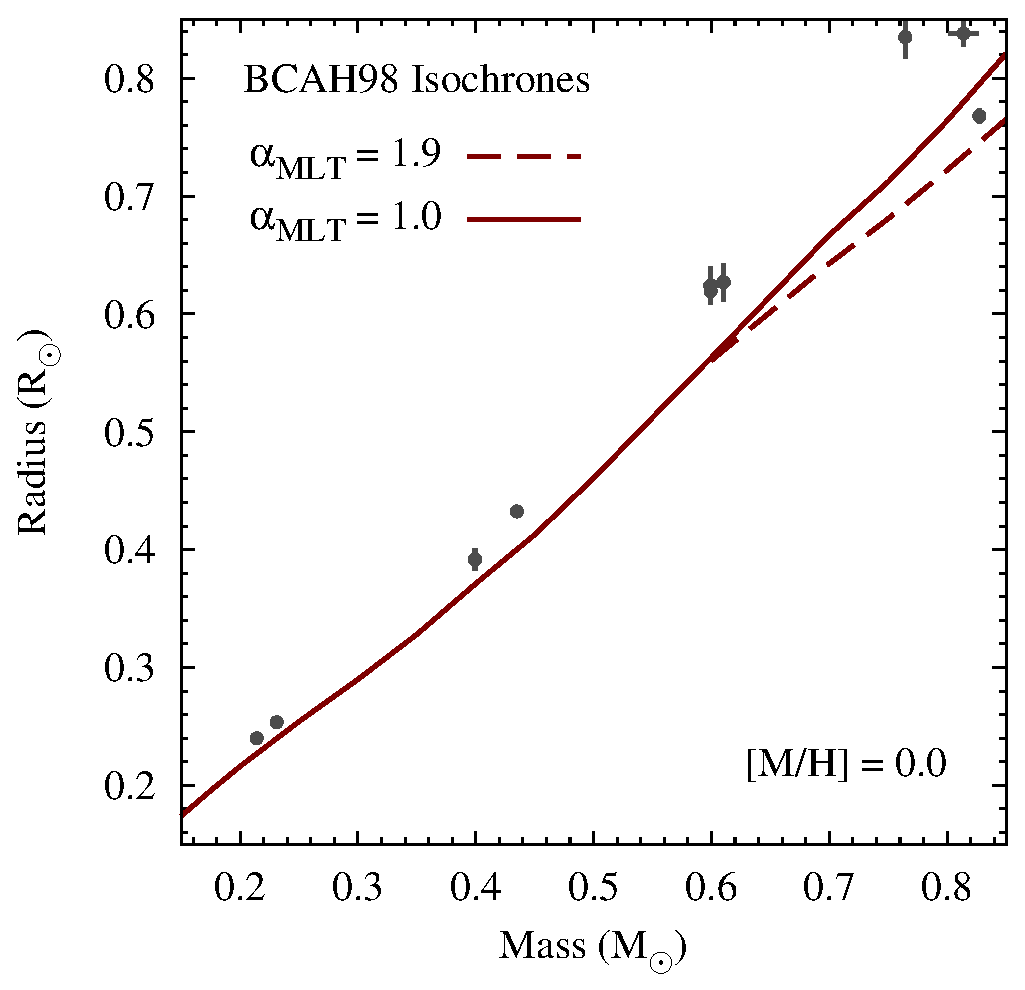
\includegraphics[scale=0.42]{./ch1/fig/bcah_1_gyr_MR.eps}
        \hspace{\fill}
        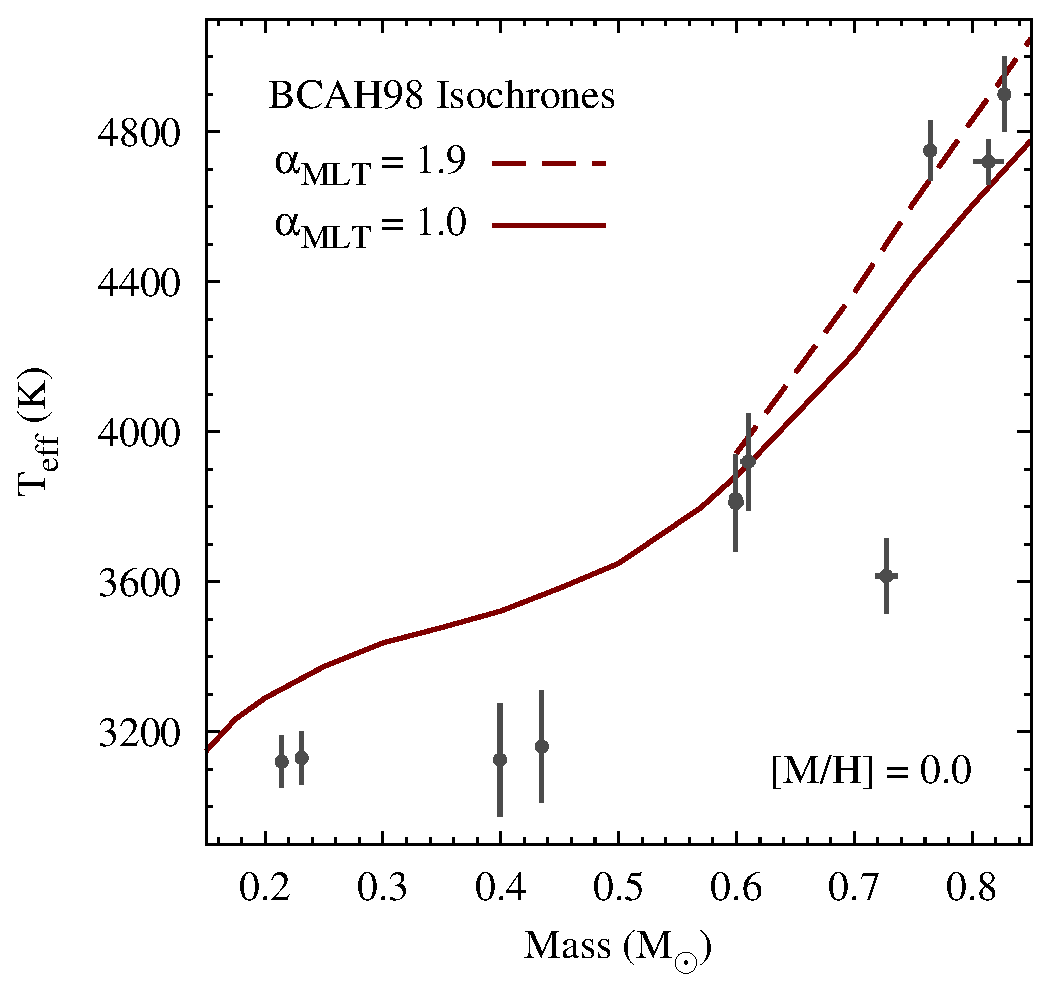
\includegraphics[scale=0.42]{./ch1/fig/bcah_1_gyr_MT.eps}
        \caption[Example of a simple figure.]
        {An example of a two panel figure. Naturally, there can 
         be as few or as many panels as you'd like. All figures 
         will be numbered Chapter.Section and will be refered to
         as such using the ``label--reference'' system. Additionally,
         there is no need for figures to be on separate pages in
         a Dartmouth thesis, it's up to the author.}
        \label{fig:example1}
    \end{center}
\end{figure}


\subsection{Sub-section Title}
\label{sec:sub}

\subsubsection{Sub-sub-section Title}
\label{sec:subsub}


   
    % Note: directory is referenced from the **top** level
    
       % Chapter 1
%------------------------------------------------------------------------%
% Example appendix chapter for the thesis template.                      %
%                                                                        %
%      Author: Gregory Alexander Feiden                                  %
%   Institute: Dartmouth College                                         %
%        Date: 2014 May 17                                               %
%                                                                        %
%     License: Beerware (revision 42)                                    %
%              ----------------------                                    %
%              Gregory Feiden wrote this file. As long as you retain     %
%              this notice you can do whatever you want with this code.  %
%              If we meet some day and you think this code is worth it,  %
%              you can buy me a beer in return.                          %
%                                                                        %
%------------------------------------------------------------------------%

\appendix

% import first appendix, note that you cannot next \includes
\newpage
%------------------------------------------------------------------------%
% Example appendix section for the thesis template.                      %
%                                                                        %
%      Author: Gregory Alexander Feiden                                  %
%   Institute: Dartmouth College                                         %
%        Date: 2014 May 17                                               %
%                                                                        %
%     License: Beerware (revision 42)                                    %
%              ----------------------                                    %
%              Gregory Feiden wrote this file. As long as you retain     %
%              this notice you can do whatever you want with this code.  %
%              If we meet some day and you think this code is worth it,  %
%              you can buy me a beer in return.                          %
%                                                                        %
%------------------------------------------------------------------------%

\chapter{Things People May Find Important}
\label{app:example1}

An example of an appendix with a landscaped long table and a snippet of
code imported from the {\it original} file.

% Example of code imported from original file.
\vspace{\baselineskip}
\onehalfspacing
\lstinputlisting[language=Fortran,caption=Sample Fortran File using Listings]
                {/home/gfeiden/evolve/nml/magnetic.nml}
\doublespacing

% Example of a big table created using longtable environment.
% Low-mass stars with direct magnetic field measurements. Data is pulled from the Reiners (2012, LRSP, 1)
% and Anderson et al. (2010, A&A, 522, A81). The Reiners review data is a compilation from other literature
% sources, primarily Reiners, Basri, & Browning (2009, 692, 538) and Reiners & Basri (2007, ApJ, 656, 1121).
%
% Compiled by: Gregory A. Feiden, Dartmouth College  <gregory.a.feiden.gr@dartmouth.edu>
%
% Notes:
% ------
% Spectral types and radii are those quoted by the original sources or were estimated based on spectral type
% using a comparison with similar star (late M) or estimation based on DSEP models (G and K stars). Parallax
% data was acquired from SIMBAD and represent the latest Hipparcos parallax estimates (van Leeuwen 2007). 
% X-ray count rates and hardness ratios are from the ROSAT All-Sky Survey Bright and Faint Source Catalogues
% (Voges et al. 1999, 2000). Conversion to X-ray fluxes was performed following the conversion defined by
% Schmitt et al. (1995).
% 
% Column headers:
% ---------------
%
% Star	    Other   SpT	    <Bf>	Radius	  Phi      log(Phi)	 Pi	     d	     Xcr	 HR1	  Fx	      Lx       log(Lx)
% Name	    Name    ()    	(kG)	(Rsun)	  (Mx)	    (Mx)	(mas)	(pc)   (cnt/s)	 ()   (erg/s/cm**2)	(erg/s)	   (erg/s)
%-------------------------------------------------------------------------------------------------------------------------------

\begin{landscape}
\onehalfspacing
\begin{center}
    \begin{longtable}{l l l c c c c c c c c} 
        \caption[Example of a table using longtable.]
         {Example of a long table in landscape mode.}
        \label{tab:lms_xray_data}\\
        
        % Define the header at the top of the first page.
        \hline
        \hline
        Star & Other & SpT & $\langle Bf \rangle$ & $R_\star$ & $\log(\Phi)$ & $\pi$ & $X_{\rm cr}$ & HR & $F_x$ & $\log(L_x)$ \\
        Name & Name & & (kG) & $(\rsun)$ & (Mx) & (mas) & $\mathrm{(cnts\, s^{-1})}$ &  & $\mathrm{(erg\, s^{-1}\, cm^{-2})}$ & $\mathrm{(erg\, s^{-1})}$ \\
        \hline
        \endfirsthead
        
        % Define the header at the top of all but the first page
        \multicolumn{11}{c}{\bf \tablename\ \thetable{} -- continued} \\
        \hline 
        \hline
        Star & Other & SpT & $\langle Bf \rangle$ & $R_\star$ & $\log(\Phi)$ & $\pi$ & $X_{\rm cr}$ & HR & $F_x$ & $\log(L_x)$ \\
        Name & Name & & (kG) & $(\rsun)$ & (Mx) & (mas) & $\mathrm{(cnts\, s^{-1})}$ &  & $\mathrm{(erg\, s^{-1}\, cm^{-2})}$ & $\mathrm{(erg\, s^{-1})}$ \\
        \hline
        \endhead
        
        % Define footer at the bottom of each page
        \hline
        \multicolumn{11}{c}{\bf \footnotesize continued on next page} \\
        \endfoot
        
        % Define footer at the bottom of the table
        \hline
        \endlastfoot
%
%  Star          Other   SpT     <Bf>      R       logPhi    Par     Xcr       HR      Fx       logLx
%  Name          Name            (kG)     (Ro)      (Mx)    (mas)   (c/s)         (erg/s/cm**2)(erg/s)
HD 115383    & 	59 Vir & G0	  &  0.5	& 0.74 &	25.22 &	56.95  & 1.12 &	-0.14 &	8.48E-12 &	29.50 \\
HD 115617    & 	61 Vir & G6	  &  0.1	& 0.95 &	24.74 &	116.89 & 0.01 &	-0.96 &	4.58E-14 &	26.60 \\
$\sigma$ Dra & 	-	   & K0	  &  0.1	& 0.80 &	24.59 &	173.77 & 0.26 &	-0.80 &	1.06E-12 &	27.62 \\
40 Eri	     &  -	   & K1	  &  0.1	& 0.75 &	24.53 &	200.62 & 0.80 & -0.28 &	5.46E-12 &	28.21 \\
$\epsilon$ Eri&  -	   & K2	  &  0.1	& 0.70 &	24.59 &	310.94 & 2.82 &	-0.44 &	1.69E-11 &	28.32 \\
LQ Hya	     &  -	   & K2	  &  2.5	& 0.70 &	25.86 &	53.70  & 2.73 &	-0.04 &	2.21E-11 &	29.96 \\
GJ 566 B     &$\xi$ Boo B& K4 &  0.5	& 0.70 &	25.14 &	149.26 & 2.44 &	-0.31 &	1.63E-11 &	28.94 \\
Gl 171.2 A   & 	-	   & K5	  &  1.4	& 0.65 &	25.56 &	55.66  & 2.69 &	-0.04 &	2.18E-11 &	29.93 \\
Gl 182	     &  -      & M0.0 &  2.5	& 0.60 &	25.74 &	38.64  & 0.65 &	-0.19 &	4.75E-12 &	29.58 \\
Gl 803	     &  AU Mic & M1.0 &  2.3	& 0.50 &	25.54 &	100.91 & 5.95 &	-0.07 &	4.72E-11 &	29.74 \\
Gl 569 A	 &  -	   & M2.0 &  1.8	& 0.40 &	25.24 &	-	   & 0.49 &	-0.40 &	3.03E-12 &    -   \\
Gl 494	     &  DT Vir & M2.0 &  1.5	& 0.40 &	25.16 &	85.54  & 1.57 &	-0.01 &	1.30E-11 &	29.33 \\
Gl 70	     &  -	   & M2.0 &  0.2	& 0.33 &	24.12 &	87.62  & 0.04 &	-0.67 &	2.08E-13 &	27.51 \\
Gl 873	     &  EV Lac & M3.5 &  3.8	& 0.31 &	25.35 &	195.22 & 5.83 &	-0.16 &	4.35E-11 &	29.14 \\
Gl 729	     &V1216 Sgr& M3.5 &  2.1	& 0.20 &	24.71 &	336.72 & 0.94 &	-0.43 &	5.67E-12 &	27.78 \\
Gl 87	     &  -	   & M3.5 &  3.9	& 0.30 &	25.33 &	96.02  & -    &   -	  &   -	     &    -   \\
Gl 388	     &  AD Leo & M3.5 &  3.0	& 0.39 &	25.44 &	213.00 & 3.70 &	-0.27 &	2.55E-11 &	28.83 \\
GJ 3379	     &  -	   & M3.5 &  2.3	& 0.25 &	24.94 &	190.93 & 0.40 &	-0.20 &	2.90E-12 &	27.98 \\
GJ 2069 B    & 	CV Cnc & M4.0 &  2.7	& 0.25 &	25.01 &	78.10  & 0.24 &	-0.14 &	1.82E-12 &	27.95 \\
Gl 876	     &  IL Aqr & M4.0 &  0.2	& 0.31 &	24.07 &	213.28 & -	  &   -	  &   -	     &    -   \\
GJ 1005 A    & 	-	   & M4.0 &  0.2	& 0.23 &	23.81 &	191.86 & -	  &   -	  &   -	     &    -   \\
Gl 490 B	 &G 164-31 & M4.0 &  3.2	& 0.20 &	24.89 &	50.00  & 0.84 &	-0.22 &	6.00E-12 &	29.46 \\
Gl 493.1	 &  FN Vir & M4.5 &  2.1	& 0.20 &	24.71 &	123.10 & 0.14 &	-0.16 &	1.04E-12 &	27.92 \\
GJ 4053	     &LHS 3376 & M4.5 &  2.0	& 0.17 &	24.55 &	137.30 & 0.06 &	-0.49 &	3.43E-13 &	27.34 \\
GJ 299	     &  -	   & M4.5 &  0.5	& 0.18 &	23.99 &	148.00 & -	  &   -	  &   -	     &    -   \\
GJ 1227	     &  -	   & M4.5 &  0.2	& 0.19 &	23.64 &	120.00 & -	  &   -	  &   -	     &    -   \\
GJ 1224	     &  -	   & M4.5 &  2.7	& 0.18 &	24.73 &	132.60 & 0.21 &	-0.45 &	1.24E-12 &	27.93 \\
Gl 285	     &  YZ Cmi & M4.5 &  4.5	& 0.30 &	25.39 &	167.88 & 1.47 &	-0.21 &	1.06E-11 &	28.65 \\
GJ 1154 A    & 	-	   & M5.0 &  2.1	& 0.20 &	24.71 &	-	   & 0.10 &	-0.23 &	7.09E-13 &    -   \\
GJ 1156	     &  GL Vir & M5.0 &  2.1	& 0.16 &	24.51 &	152.90 & 0.13 &	-0.25 &	9.08E-13 &	27.67 \\
Gl 905	     &  HH And & M5.5 &  0.1	& 0.17 &	23.24 &	316.70 & 0.18 &	0.15  & 1.64E-12 &	27.29 \\
GJ 1057	     &  CD Cet & M5.5 &  0.1	& 0.18 &	23.29 &	117.10 & -	  &   -	  &   -	     &    -   \\
GJ 1245 B    & 	-	   & M5.5 &  1.7	& 0.14 &	24.31 &	220.00 & 0.20 &	-0.37 &	1.27E-12 &	27.50 \\
GJ 1286	     &  -	   & M5.5 &  0.4	& 0.14 &	23.68 &	138.30 & -	  &   -	  &   -	     &    -   \\
GJ 1002	     &  -	   & M5.5 &  0.2	& 0.13 &	23.31 &	213.00 & -	  &   -	  &   -	     &    -   \\
Gl 406	     & CN Leo  & M5.5 &  2.4	& 0.13 &	24.39 &	418.30 & 0.23 &	-0.22 &	1.64E-12 &	27.05 \\
Gl 412 B	 &  WX Uma & M6.0 &  3.9	& 0.13 &	24.60 &	206.94 & 0.18 &	-0.64 &	8.85E-13 &	27.39 \\
GJ 1111	     &  DX Cnc & M6.0 &  1.7	& 0.12 &	24.17 &	275.80 & -	  &   -	  &   -	     &    -   \\
Gl 644C	     &  VB 8   & M7.0 &  2.3	& 0.10 &	24.15 &	153.96 & -	  &   -	  &   -	     &    -   \\
GJ 3877	     &LHS 3003 & M7.0 &  1.5	& 0.10 &	23.96 &	157.80 & -	  &   -	  &   -	     &    -   \\
GJ 3622	     &  -	   & M7.0 &  0.6	& 0.10 &	23.56 &	221.00 & -	  &   -	  &   -	     &    -   \\
LHS 2645	 &  -      & M7.5 &  2.1	& 0.08 &	23.91 &	-	   & -	  &   -	  &   -	     &    -   \\
LP 412-31    & 	-	   & M8.0 &  3.9	& 0.08 &	24.18 &	-	   & -	  &   -	  &   -	     &    -   \\
VB 10	     &V1298 Aql& M8.0 &  1.3	& 0.08 &	23.70 &	164.30 & -	  &   -	  &   -	     &    -   \\
LHS 2924	 &  -	   & M9.0 &  1.6	& 0.08 &	23.79 &	90.00  & -	  &   -	  &   -	     &    -   \\
LHS 2065	 &  -	   & M9.0 &  3.9	& 0.08 &	24.18 &	116.80 & -	  &   -	  &   -	     &    - 
    \end{longtable}
\end{center}
\end{landscape}

\doublespacing



       % Appendicies A & B
%--- END CHAPTERS

% Bibliography using bibtex & natbib w/ MNRAS style formatting
\clearpage
\addcontentsline{toc}{chapter}{Bibliography}
\bibliographystyle{mn}
\bibliography{/directory/structure/papers.bib}

\end{document}
%--- END THESIS DOCUMENT


%=== END OF FILE
